\documentclass[a4paper, 12 pt]{article}

\usepackage[english, russian]{babel}
\usepackage[T2A]{fontenc}
\usepackage[utf8]{inputenc}
\usepackage{graphicx}
\usepackage[unicode, pdftex]{hyperref}
\usepackage{amssymb}
\DeclareGraphicsExtensions{.png, .pdf}
\begin{document}
	\pagestyle{plain}
	\begin{center}
		\large МИНИСТЕРСТВО НАУКИ И ВЫСШЕГО ОБРАЗОВАНИЯ РОССИЙСКОЙ ФЕДЕРАЦИИ\
		\vspace*{5mm}
		
		\small ФЕДЕРАЛЬНОЕ ГОСУДАРСТВЕННОЕ АВТОНОМНОЕ ОБРОЗОВАТЕЛЬНОЕ УЧРЕЖДЕНИЕ ВЫСШЕГО ОБРАЗОВАНИЯ
		\mbox{\guillemotleft Национальный исследовательский институт ИТМО\guillemotright}
		\vspace*{10mm}
		
		\mbox{ФАКУЛЬТЕТ ПРОГРАМНОЙ ИНЖЕНЕРИИ И ВЫЧИСЛИТЕЛЬНОЙ ТЕХНИКИ}
		\vspace*{5mm}
		
		{\bf ЛАБОРАТОРНАЯ РАБОТА №4}
		\linebreak
		по дисциплине
		\linebreak
		\guillemotleft ИНФОРМАТИКА\guillemotright
		\linebreak
		\large Вариант №7
		\vspace*{50mm}
		
	\end{center}
	
	
	\begin{flushright}
		\textbf{\textit{Выполнил:}}
		\linebreak
		Студент группы P3118
		\linebreak
		Михайлов Дмитрий
		\linebreak
		Андреевич
		\linebreak
		\textbf{\textit{Преподаватель:}}
		\linebreak
		Рыбаков Степан
		\linebreak
		Дмитриевич
		\vspace*{30mm}
		
	\end{flushright}
	\begin{center}
		\small Санкт-Петербург, 2022
	\end{center}
	\thispagestyle{empty}
	\newpage
	
	\begin{flushleft}
		\textbf{\LARGE \section{Содержание}}
		\subsection{Задание........................................................3}
		\subsection{Основные этапы выполнения......................4 - 5}
		\subsection{Вывод...........................................................6}
		\subsection{Список литературы.....................................7}
	\end{flushleft}
	\newpage
	
	\begin{flushleft}
		\textbf{\LARGE 1.1 Задание.}
		\linebreak
		\LARGE Вариант №7
		\linebreak
		\vspace*{5mm}
	\end{flushleft}

	\begin{center}
		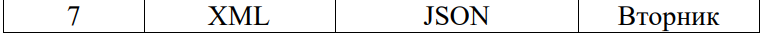
\includegraphics{Task}
		\captionsrussian{\small Рис. 1, Вариант задания.}
		\vspace*{10mm}
	\end{center}

	\begin{center}
		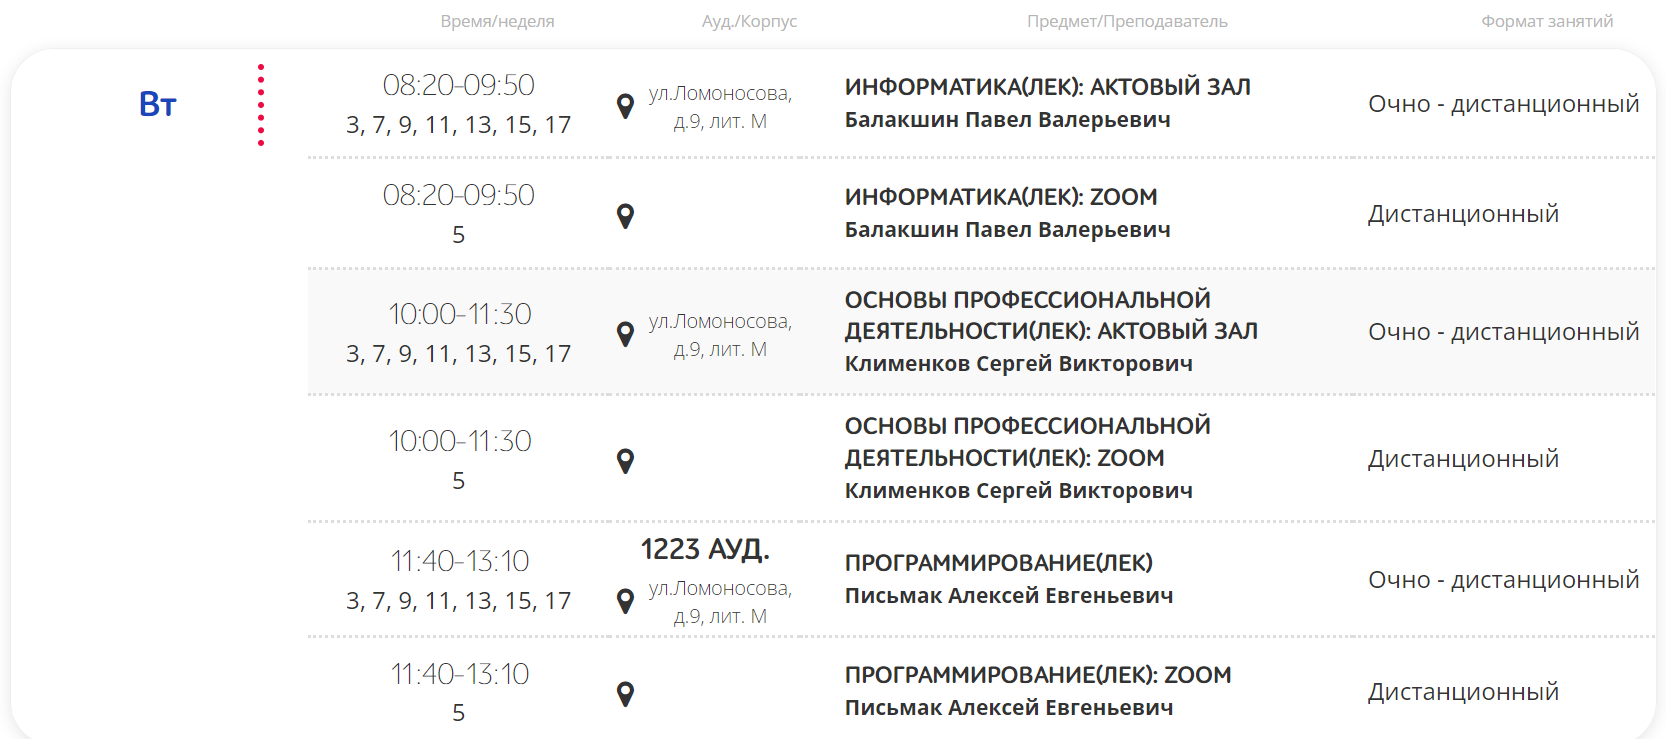
\includegraphics[scale=0.5]{Schedule}
		\captionsrussian{\small Рис. 2, Расписание на день недели из варианта.}
	\end{center}
	\setcounter{page}{3}

	\newpage
	\begin{flushleft}
		\textbf{\LARGE 1.2 Основные этапы выполнения.}
		\linebreak
		\vspace*{5mm}
		
		\small Для начала, нам необходимо записать расписание в файл формата \textbf{XML}.
		\linebreak
		\small Ознакомясь с синтаксисом языка разметки \textbf{XML}, записываем наш исходник.
		\linebreak
		\small Для решения задачи, нам необходимо также понять, что такое парсинг.
		\linebreak
		\small \textit{Парсинг} (по-русски <<синтаксический анализ>>) - понятие синтаксиса языка, изъятие информации, понимание синтактического дерева файла.
	\end{flushleft}
	
	\begin{center}
		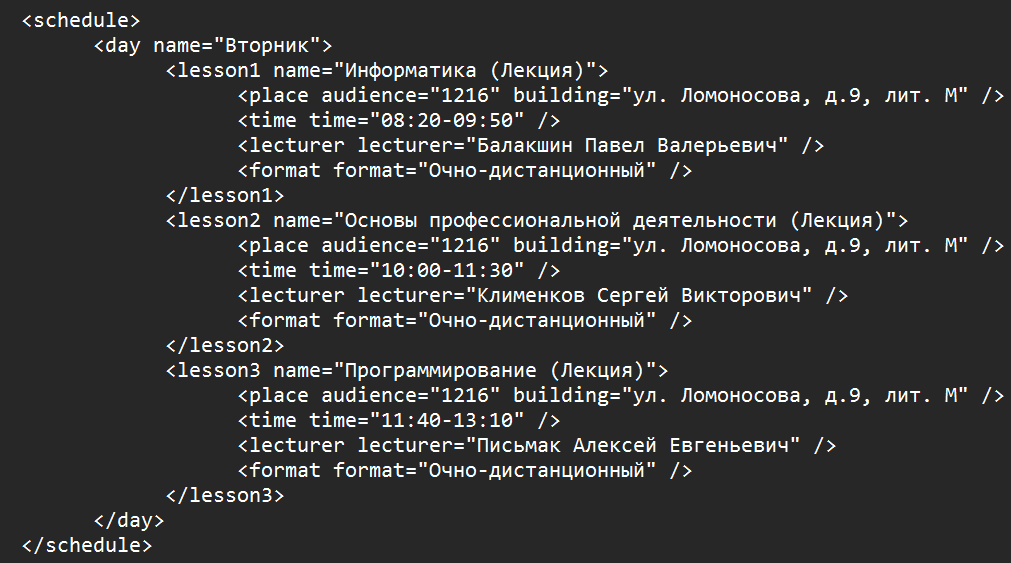
\includegraphics[scale=0.8]{xml}
		\captionsrussian{Рис. 3, Исходный XML файл.}
		\vspace*{10mm}
	\end{center}
	
	\begin{flushleft}
		\href{https://github.com/mysticslippers/Lab4_INF}{\textbf{\LARGE Репозиторий с иходным кодом для основного и дополнительных заданий.}}
	\end{flushleft}
	\newpage
	
	\begin{flushleft}
		\small После преобразования исходного файла различными путями, наш результирующий файл получается всегда таким:
		\linebreak
	\end{flushleft}
	
	\begin{center}
		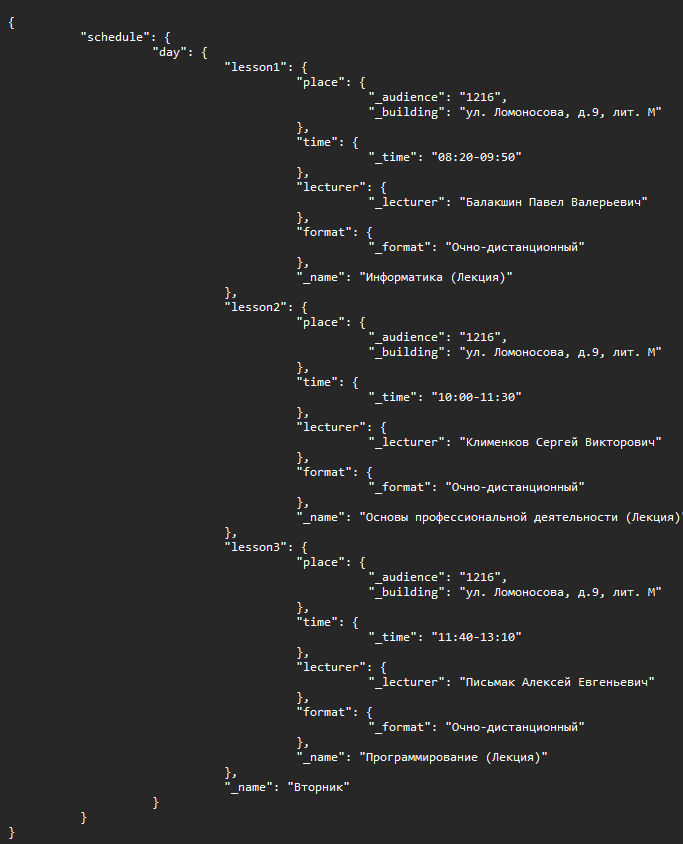
\includegraphics[scale=1]{json}
		\linebreak
		\captionsrussian{Рис. 4, Результат работы программы в формате json.}
	\end{center}
	\newpage
	
	\begin{flushleft}
		\textbf{\LARGE 1.3 Вывод.}
		\linebreak
		\vspace*{5mm}
		
		 Выполняя данную лабораторную работу, я ознакомился с таким понятием, как парсинг, с синтаксисом нескольких языков разметки. Я уверен, что мне это пригодится в будущем.
	\end{flushleft}
	\newpage
	
	\begin{flushleft}
		\textbf{\LARGE 1.4 Список литературы.}
		\linebreak
		\vspace*{5mm}
		
		\small 1. Лямин А.В., Череповская Е.Н. Объектно-ориентированное программирование. Компьютерный практикум. – СПб: Университет ИТМО, 2017. – 143 с. – Режим доступа:
		\href{https://books.ifmo.ru/file/pdf/2256.pdf}{https://books.ifmo.ru/file/pdf/2256.pdf}
		\linebreak
		\small 2. Статья <<Пишем изящный парсер на Питоне>> - Режим доступа:
		\href{https://habr.com/ru/post/309242/}{https://habr.com/ru/post/309242/}
	\end{flushleft}
\end{document}